%%%%%%%%%%%%%%%%%%%%%%%%%%%%%%%%%%%%%%%%%%%%%%%%%%%%%%%%%%%%%%%%%%%%%%%%
%%%%%                                                              %%%%%
%%%%% Chapter 2: Background                                        %%%%%
%%%%%                                                              %%%%%
%%%%%%%%%%%%%%%%%%%%%%%%%%%%%%%%%%%%%%%%%%%%%%%%%%%%%%%%%%%%%%%%%%%%%%%%
\chapter{Background}
\label{ch2}

%%%%%%%%%%%%%%%%%%%%%%%%%%%%%%%%%%%%%%%%%%%%%%%%%%%%%%%%%%%%%%%%%%%%%%%%
%%%%%%%%%%%%%%%%%%%%%%%%%%%%%%%%%%%%%%%%%%%%%%%%%%%%%%%%%%%%%%%%%%%%%%%%
%%%%%%%%%%%%%%%%%%%%%%%%%%%%%%%%%%%%%%%%%%%%%%%%%%%%%%%%%%%%%%%%%%%%%%%%
\section{Nanopore sequencing}
%% Intro

%%% History of nanopore development
\paragraph{A brief history of nanopore sequencing}
%% Initial idea and expreiments
The concept of nanopore sequencing is based on the idea that as a
single-stranded DNA (or RNA) translocates through a nanometer sized
pore, a nanopore, in the presence of an electric field, the change in
current level measured across the nanopore would be dependent on the
nucleotide passing through the nanopore; thus, measuring the current
over time could be leveraged to determine the sequence of nucleotides
(Fig.~\ref{nanopore}a).
%
This idea of using transmemberane proteins an nanopores for sensing and
sequencing nucleic acids was independently thought of by several
researches including David Deamer, Hagan Bayley, and George Church
\citep{deamer2016three,bayley2015nanopore,branton2010potential}.

%% Initial expreiments
% Detecting the presence of oligos
Initial experiments showed that as a single-stranded DNA or RNA
molecules could be driven through a \emph{Staphylococcus aureus}
$\alpha$-hemolysin in the presence of an electric field
\citep{kasianowicz1996characterization}. The current through the pore
remained constant in the absence of oligomers; and the presence of
oligomers caused transient decreases in current, with the duration of
the decrease proportional to the length of the oligomer.
% Detecting the bases in oligos
Further research demonstrated that decrease in amplitude of current
could be used to differentiate between poly-purine and poly-pyrimidine
sequences of RNA \citep{akeson1999microsecond} and DNA
\citep{meller2000rapid}. It was also observed that the DNA molecules
translocate through the nanopore at few microseconds per base
\citep{meller2000rapid}.

\begin{figure}[b!]
\centering
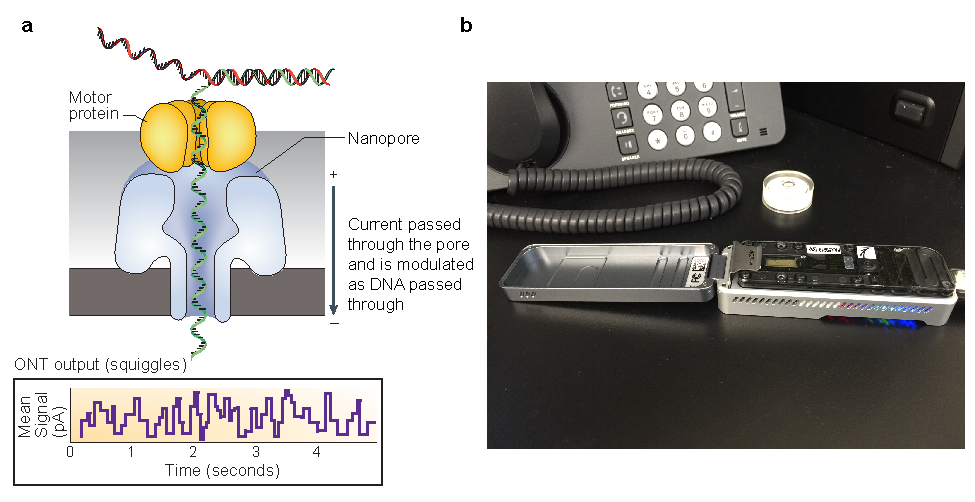
\includegraphics{nanopore.pdf}
\caption[Nanopore sequencing]{
  Nanopore sequencing.
  (a) Change in current across a nanopore is measured as a DNA molecule
  translocates through a nanopore. This figure is
  adapted from Figure 5Ab in \cite{goodwin2016coming}.
  (b) Oxford Nanopore Technologies MinION instrument.}
\label{nanopore}
\end{figure}

%% Challenges for sequencing DNA
Although these experiments demonstrated the potential for nanopores to
distinguish nucleic acid polymers, several challenges remained to be
addressed to use this approach for reading individual bases on a DNA or
RNA molecule.
%
The most important of these were detecting the bases at a single
nucleotide resolution and slowing the rate of translocation through the
nanopore so that a readout can be obtained
\citep{bayley2015nanopore,branton2010potential}.
%
These challenges were resolved in the forthcoming years. A few notable
milestones are described below.

%% Single nucleotide detection
In regard to identifying individual nucleobases, all four bases were
identified in a single-stranded DNA that had a terminal hairpin
structure \citep{ashkenasy2005recognizing} and single-stranded DNA
attached to streptavidin with a biotin linker
\citep{purnell2009discrimination,stoddart2009single}. These structures
immobilized the DNA in the nanopore (either a wildtype
$\alpha$-hemolysin or an engineered form of it) allowing sufficient time
for detection. Thus, with the appropriate sequence, each base could be
resolved, and further, the location within a nanopore that is most
sensitive to detect bases was also determined.


%% engineered nanopores
The frequency of translocation of DNA molecules through a
$\alpha$-hemolysin pore was increased and the voltage threshold for
translocation was decreased by engineering the pore to have positive
charged groups in the lining of the lumen \citep{maglia2008enhanced}.
%
However, a disadvantage of the $\alpha$-hemolysin pores is that the
region that is sensitive to the nucleotides in the pore is too wide, and
so the current differences are small between nucleotides, making single
nucleotide detection difficult.
%
Pores derived from \emph{Mycobacterium smegmatis} porin A have a
narrower sensitive region, and could detect nucleotides at a higher
resolution \citep{butler2008single,manrao2011nucleotide}.

%% processivity control
In regard to controlling the rate of translocation through a nanopore,
there were two approaches, exo-sequencing and strand-sequencing.
% exo-sequencing
In the exo-sequencing approach, individual bases from a DNA are cleaved
into a nanopore with an exonuclease and identified one at a time
\citep{astier2006toward,clarke2009continuous}.
% strand-sequencing
Alternatively, in the strand sequencing approach a DNA molecule is
threaded though a nanopore at a controlled rate and the bases are
identified from the continuous change in current levels. Initial
approaches in strand sequencing used a DNA polymerase (derived from
\emph{Escherichia coli} Kleenow fragment or bacteriophage T7) and
recorded the current levels as the DNA translocates through a pore with
the incorporation of each nucleotide
\citep{benner2007sequence,cockroft2008single,gyarfas2009mapping,
chu2010real}.
%
Subsequently it was shown that $\phi$29 polymerase could be used to control
ratcheting in both the forward and the reverse direction
\citep{lieberman2010processive,manrao2012reading,cherf2012automated}.
$\phi$29 was used to sequence reads up to 4.5 kb from the $\phi$X174 genome
using nanopores \citep{laszlo2014decoding}.


%% Oxford nanopore technologies
\paragraph{Oxford Nanopore Technologies}
Oxford Nanopore Technologies was founded in 2005 by Hagan Bayley and
colleagues \citep{deamer2016three}. Oxford Nanopore Technologies
announced the MinION instrument at the Advances in Genome Biology and
Technology meeting in 2012 and made it available to early access
researches in 2014 \citep{deamer2016three,bayley2015nanopore}.

%% Oxford MinION
The MinION sequencer (Fig.~\ref{nanopore}b) is a portable instrument
requiring just a modest computer for control and data acquisition.  A
MinION flowcell consists of 2,048 nanopores (at present, a derivative of
\emph{Escherichia coli} CsgG protein \citep{brown2016nanopore}) embedded
on a membrane, of which 512 pores can sequence molecules in parallel.

%% Current state of nanopore sequencing
Whole genomes of several organisms including humans have been sequenced
using the MinION instrument \citep{loman2015complete,stancu2017mapping,
jain2018nanopore,bowden2019sequencing,moss2020complete}. It has also
been used in several other applications such as disease surveillance
\citep{quick2016real,faria2016mobile}, metagenomics
\citep{goordial2017situ,charalampous2019nanopore,leggett2020rapid},
direct RNA sequencing \citep{garalde2018highly,workman2019nanopore,
depledge2019direct}, and detecting methylated bases
\citep{rand2017mapping,simpson2017detecting,liu2019accurate}, among
others \citep{jain2016oxford}.

%% other decives from ONT
In addition to the MinION instrument, Oxford Nanopore Technologies
currently offers various nanopore devices including the bench-top
GridION and PromethION which allow for parallel sequencing with up to 5
and 48 flowcells, respectively.


%% Nanopore library construction
\paragraph{Nanopore library preparation and sequencing}
Sequencing nucleic acids requires preprocessing the sample DNA for
compatibility with the underlying sequencing technology, a process
traditionally referred to as library preparation.
%
Sequencing on a nanopore machine usually requires fragmenting DNA
molecules to the appropriate length and attaching sequencing adapters.
%
Oxford Nanopore Technologies offers several commercially library
preparation kits for both DNA and RNA samples.  Of the available kits,
most commonly used are the ligation sequencing kit family and the rapid
sequencing kit family.

% Ligation kit
In theory, there is no limit on the length of a molecule that can be
sequenced with a nanopore, and thus, the length is determined by the
downstream application or the limitations of handling high molecular
weight DNA. For the ligation sequencing kit (SQK-LSK108 1D DNA by
ligation), the recommended length is $\sim$8 kb when starting with
\SI{1}{\micro\gram} of sample to ensure appropriate molar concentration
in the subsequent steps.  DNA molecules can be fragmented to the
appropriate length using a variety of methods including the Covaris
g-TUBE.
%
These molecules are then optionally repaired to remove any nicks, and
then the DNA ends are prepared to have a dA tail. Finally, sequencing
adapters (that have a dT tail) are ligated to the end-prepared DNA.
These adapters contain specific DNA sequenced with attached enzymes that
regulate translocation of the DNA molecule into a nanopore.  Library
preparation with the ligation kit takes approximately 60 minutes.

% Rapid kit
The rapid library preparation kit (SQK-RAD003 Rapid sequencing) offers a
faster method, by simultaneously fragmenting and tagging the ends of
high molecular weight DNA (recommended $>$ 30 kb). Adapters are then
attached to these tags.  Library preparation with the rapid kit takes
approximately 10 minutes.

% Barcoding capablities
Both of these kits offer barcoding capabilities for multiplexing several
samples in a single sequencing run. For example, the native barcode kit
(EXP-NBD103) is used together with the ligation sequencing kit, and
adds a barcode sequence to the end-prepared DNA molecules prior to
ligating sequencing adapters. After library preparation with a unique
barcode for each sample, they are pooled in appropriate molar
concentrations before sequencing.

% Brief summary of other kits
Oxford Nanopore Technologies offers several other preparation kits, such
as the $\text{1D}^2$ kit for higher accuracy reads and PCR based kits when
starting with nanogram or picogram amounts of DNA.

% After lib. prep.: loading and sequencing
After library construction the sample is ready to be sequenced. The
flowcell is loaded on the sequencing machine, primed with the appropriate
buffers, and the sample is loaded. After which the sequencing can be
started and the reads are available as they are sequenced in real-time.
%
The sequencing process is controlled by the MinKNOW tool, and can
continue for up to 48 hours.
% Base-calling reads
The sequenced reads are converted from current level ``squiggles'' into
base-space using base-calling tools such as Guppy (Oxford Nanopore
Technologies).

%% Properties of nanopore reads
% Read length
Reads generated from a sequencing run are typically several kilobases
long.
% idintity
At present, the reads sequenced with the 1D protocol align with
approximately 85\% identity to the reference genome
\citep{bowden2019sequencing,jain2018nanopore,carter2017robust}.  The
accuracy of reads are a continually improving with improvements to both
the nanopore and the base-calling tools.
% GC-bias
Nanopore sequencing does not introduce significant a GC bias when the
samples are prepared with a protocol that does not use PCR
\citep{carter2017robust}.


%%%%%%%%%%%%%%%%%%%%%%%%%%%%%%%%%%%%%%%%%%%%%%%%%%%%%%%%%%%%%%%%%%%%%%%%
%%%%%%%%%%%%%%%%%%%%%%%%%%%%%%%%%%%%%%%%%%%%%%%%%%%%%%%%%%%%%%%%%%%%%%%%
%%%%%%%%%%%%%%%%%%%%%%%%%%%%%%%%%%%%%%%%%%%%%%%%%%%%%%%%%%%%%%%%%%%%%%%%
\section{Copy number variation and profiling}
%% Background
\paragraph{Copy number variation}
% genetic variations
Sources of genomic variation in humans include single-nucleotide
polymorphisms (SNPs), short insertions and deletions, and variable
number tandem repeats.
% CNV
Another source of variation, copy number variation (CNV), is the change
in number of copies of a region of the genome larger than 1 kb with
respect to a reference genome
\citep{redon2006global,feuk2006structural}.  The number of copies of a
region of the genome could increase resulting in a copy number ``gain''
(also referred to as amplification or duplication), or decrease
resulting in a copy number ``loss'' (also referred to as deletion).
% source of cnv
Changes in copy number can occur due to mechanisms such as homologous
recombination and non-homologous DNA repair mechanisms
\citep{hastings2009mechanisms,van2011origins,stankiewicz2010structural}.

% initial studies
% copy number polymorphisms
Copy number variations contribute both to diversity in the human
population and to disease.
% Germline and somatic cnv
Variations that contribute to diversity are present in the germline,
whereas those that contribute to diseases could in the germline or
somatic. (Somtic copy number variations, especially when realted to
cancer, are referred to as somatic copy number alterations or
CNA, in short.)

% cnv in diversity
\paragraph{Copy number variation in diversity}
CNVs as a significant source of diversity in humans was established by
\cite{sebat2004large} and \cite{iafrate2004detection}.
%
\cite{sebat2004large} identified 221 copy number differences in 20
individuals with an average of 11 differences between individuals; these
variations had an average length of 465 kb (median length of 222 kb).
%
\cite{iafrate2004detection} identified 225 regions in 55 individuals
with an average of 12.4 differences between individuals; these
variations ranged from 150 kb to 425 kb.
%
These studies were extended to larger populations and to populations of
different ancestry \citep{redon2006global,li2009whole}.  CNVs in the
human genome and those that contribute to diversity are reviewed in
\citep{freeman2006copy,feuk2006structural,zarrei2015copy}.

%% CNV in diseases
\paragraph{Copy number variation in diseases}
Changes in copy number of genes or whole chromosomes are implicated in
several diseases. The most notable example is the trisomy of chromosome
21 in Down's syndrome \citep{antonarakis2004chromosome}.
%
Mechanisms by which copy number variations alter phoenotype include:
over-expression of amplified genes and under-expression of deleted
genes (gene dosage effects), unmasking of a mutant recessive allele
after deletion of dominant allele, altered expression of gene that
overlaps a structural variation (such as a inversion, translocation, or
deletion), or a structural variation could disrupt regulatory elements
of a gene \citep{feuk2006structural}.
%
Changes in copy number are associated with autism
\citep{sebat2007strong}, sporadic schizophrenia \citep{xu2008strong},
psoriasis \citep{hollox2008psoriasis}, susceptibility to HIV-1/AIDS
\citep{gonzalez2005influence}, and several other diseases
\citep{stankiewicz2010structural,fanciulli2010gene}.

%% CNV in cancer
\paragraph{Copy number alterations in cancer}
Evolution of a ``normal'' single cell into a ``tumor'' cell, a tumor
cell into a mass of cells, into sub-clones of cells, and into metastatic
tumor cells all involve genomic changes to the cells
\citep{stratton2009cancer}. Of the possible genomic changes, somatic copy
number alterations play a significant role
\citep{beroukhim2010landscape,zack2013pan}.

%% Application of CNA profiling of cancer
Applications of CNA profiling of cancer can be broadly classified into
two categories, understanding the biology of cancer, and diagnostic and
prognostic evaluation of tumors. These categories are not mutually
exclusive and the advance in one drives advances in the other.

%% CNA profiling for understanding cancer
CNA profiling for understanding the biology of cancer typically involve
profiling and analyzing a collection of tumor samples within or across
cancer types.
%
CNA profiles exhibit several recurrent alterations that occur in a
significant fraction of samples within a population. These recurrent
alterations are considered to be ``driver'' alterations and play an
active role in tumor progression; whereas alterations that are unique to
few samples are considered to be ``passenger'' alterations which are
neutral to the evolution of tumor \citep{bignell2010signatures,
beroukhim2010landscape}.
%
These frequently altered driver alterations are identified from regions
on the genome that are frequently gained or lost above a significance
threshold in a population of cancer samples \citep{mermel2011gistic2}.
%
Driver alterations play significant roles in tumor progression
\citep{bignell2010signatures, beroukhim2010landscape}.  Several studies
have identified recurrent alteration in different tumor types
\citep{beroukhim2007assessing,etemadmoghadam2009integrated,
weir2007characterizing,lin2008modeling}.



%% CNA profiling in diagnostic applications
CNA profiling for diagnostic and prognostic applications would involve
profiling a tumor from a patient, and making treatment decisions based
on prior knowledge of copy number alterations.
%
These could include deciding the effectiveness of treatment and
predicting the survival of breast cancer patients
\citep{stuart2009linking,hicks2006novel}.
% Effectiveness of treatment and drug resistance
Amplification of chromosome 19q12 and 20q11.22-q13.12 is associated with
poor response to platinum-based chemotherapy and survival in ovarian
carcinomas \citep{etemadmoghadam2009integrated}.
%
Recurrent alterations are associated with gains of oncogenes and loss of
tumor suppressor genes. For example, gain of \emph{MYC}, and loss of
\emph{PTEN} and \emph{RB1} play important roles in prostate cancer
\citep{alexander2018utility}.
%
The expression of several genes in these altered regions are correlated
with the gain or loss of genomic region harboring the gene
\citep{pollack2002microarray,chitale2009integrated,lu2011integrated}.
%
Few studies have directly linked the alteration in CNA profiles with
diagnostic outcomes \citep{etemadmoghadam2009integrated,
bardelli2013amplification,berry2018genomic}, and several others have
shown that the expression level of these genes are associated with tumor
progression and response to treatment \citep{shattuck2008met,
gorre2001clinical,villanueva2013concurrent}.

%% Liquid-biopsy
In the recent years, ``liquid biopsies'' are increasingly used for
cancer screening. As opposed to a tumor biopsy (that is derived from the
tumor mass), a liquid biopsy is derived from analytes in body fluids.
Sources include extra-cellular DNA (called cell-free DNA or cfDNA)
extracted from blood serum or plasma
\citep{leary2012detection,chan2013cancer,li2017cell} or other fluids
such as aqueous humor \citep{berry2017potential} and cerebrospinal fluid
\citep{mouliere2018detection}, circulating tumor cells
\citep{dago2014rapid}, and extra-cellular RNA
\citep{zaporozhchenko2018potential}.  (Use of liquid biopsies in cancer
is reviewed in \citep{heitzer2019current,crowley2013liquid,
schwarzenbach2011cell}.)
%
Among others, an enormous advantage of a liquid biopsy is the minimally
invasive procedure used to obtain the analyte, which could be as simple
as a blood draw \citep{heitzer2019current}.
%
CNA profiles obtained from a liquid biopsy has been shown to be
concordant with profiles obtained from a solid biopsy of the same
patient \citep{chan2013cancer,berry2017potential}.
%
Gain of chromosome 6p in CNA profile generated from cfDNA samples is
predictive of eye enucleation in retinoblastoma
\citep{berry2018genomic}.
%
Moreover, other properties of cfDNA such the fraction of cfDNA molecules
from the tumor (tumor fraction) and length distribution of cfDNA
molecules are useful for tumor evaluation \citep{choudhury2018tumor,
mouliere2018enhanced,underhill2016fragment,cristiano2019genome}.  For
example, cfDNA tumor faction is associated with number of bone
metastasis in prostate cancer \citep{choudhury2018tumor}.


%% Methods for CNA profiling
\paragraph{CNA profiling methods}
%% Prior to sequencing
% microarray techniques
Initial copy number analysis, prior to high-throughput sequencing,
primarily used microarrays based techniques \citep{carter2007methods},
these include the use of comparative genome hybridization
\citep{pinkel1998high}, SNP arrays \citep{nannya2005robust}, and
oligonucleotide arrays \citep{lucito2003representational}.

%% Sequencing approaches
With the advent of high-throughput sequencing, array based approaches
are increasingly replaced with sequencing based approaches.  Techniques
for detecting copy number alterations with whole-genome sequence data
include paired-end read approach \citep{korbel2007paired,
campbell2008identification} and read-counting approach
\citep{yoon2009sensitive}.  The most commonly used, especially for tumor
samples, is the read-counting approach, and this approach can also be
used with whole-exome sequence data \citep{krumm2012copy,d2016enhanced}.

% read counting princple
Read-counting approach is based on the principle that the number of
reads originating from a region of the genome is directly proportional
to the copy number that region \citep{baslan2015optimizing}.
%
Tools for detecting copy number changes based on this approach typically
use variations of the following steps:
%
(1) Align the reads to the reference genome using any standard mapping
tool.
%
(2) Partition the genome into non-overlapping ``bins'' and determine
the number of reads mapped to each bin. The size of the bins determine
the resolution of copy number profile; small bins generate
high-resolution profiles, but also require more reads. For cancer, the
size of the copy number alterations are typically in the megabase base
range for focal alterations or chromosomal arm lengths for broad
alterations \citep{beroukhim2010landscape}, and thus, it is common to
use bins that are larger than 100 kb.
%
(3) Normalize bin counts to remove the effect of any bias that may have
been introduced. Bin counts are usually corrected for GC bias and
mappability bias. GC bias could be introduced due to PCR in the library
construction step or due to the sequencing process
\citep{aird2011analyzing,benjamini2012summarizing}. Mappability bias is
introduced as bins have unequal number of uniquely mappable positions.
%
(4) Finally, bin counts are segmented to reduce noise and determine
regions of uniform copy number. Frequently used approaches include
circular binary segmentation
\citep{olshen2004circular,venkatraman2007faster} and hidden markov
models \citep{ha2014titan}.

% tumor fraction, subclonality, and ploidy
Tumors consist of a mix of several cell types including various clones
of tumor cells, non-tumor cells in the tissue microenvironment, and
immune cells \citep{witz2006tumor}.
%
Due to which the tumor fraction of samples vary significantly
\citep{carter2012absolute,van2010allele,oesper2013theta}. Tumor fraction
varies across cancer types, with a significant number of lung,
esophageal, and breast cancer samples having under 50\% tumor fraction
\citep{carter2012absolute}.
%
In addition to detecting copy number alterations with low-coverage
sequencing, tumor fraction, subclonality, and ploidy of a tumor can also
be determined \citep{adalsteinsson2017scalable,gusnanto2012correcting}



%%%%%%%%%%%%%%%%%%%%%%%%%%%%%%%%%%%%%%%%%%%%%%%%%%%%%%%%%%%%%%%%%%%%%%%%
%%%%%%%%%%%%%%%%%%%%%%%%%%%%%%%%%%%%%%%%%%%%%%%%%%%%%%%%%%%%%%%%%%%%%%%%
%%%%%%%%%%%%%%%%%%%%%%%%%%%%%%%%%%%%%%%%%%%%%%%%%%%%%%%%%%%%%%%%%%%%%%%%
\section{Prior protocols based on concatenating DNA molecules}
%%% SAGE
% \paragraph{Serial analysis of gene expression (SAGE)}
The concept of ligating short DNA molecules prior
to sequencing was introduced in serial analysis of gene expression
(SAGE), a technique to detect thousands of expressed sequence
tags for transcript analysis \citep{velculescu1995serial}.
% principals of SAGE
SAGE technique is based on the principle that a short nucleotide sequence
tag ($\sim$ 9bp) from a defined region of a transcript has sufficient
information to uniquely identify the transcript, and the concatenation
of the short tags allows efficient analysis by sequencing multiple tags
in a single clone. The expression levels of a transcripts are then
quantified by ``counting'' the number of tags for each transcript
\citep{velculescu1995serial}.
%

%% SAGE protocol
% cDNA synthesis
Briefly, to quantity mRNA abundance using SAGE, double-stranded cDNA
molecules are synthesized from mRNA using biotinylated oligo(dT) primers.
% Anchoring enzyne digestion
These cDNA molecules are fragmented with a restriction enzyme (anchoring
enzyme).
%
After digestion, the 3' end of cDNA molecules (from the dA tail to the
anchoring enzyme recognition site) are isolated with streptavidin beads
that bind to the biotinylated oligo(dT) primers.
%
The isolated molecules are divided into two groups, and each group is
ligated to a different linker (linker A and B, respectively) using the
overhangs after the anchoring enzyme digestion. These linkers are
designed to contain a type IIS restriction site (types IIS restriction
enzymes cut $~\sim$20 bp away from a recognition site).
%
These molecules are then digested with a type IIS enzyme (tagging
enzyme) releasing the linker and a 9 bp tag.
%
The molecule from both the pools are ligated with one another to form
ditags. Ditags have linker A one end, linker B on the other, and two 9
bp tags in the middle.
%
Ditags are then PCR amplified with the primer binding sites located in
the linkers.
%
These molecules are then cleaved again with the anchoring enzyme to
remove the linkers, and leaving behind ditags with the anchoring enzyme
overhangs.  These ditags are then ligated to form longer molecules
that contain several ditags punctuated by the anchoring enzyme site.
%
The concatenated molecules are cloned and sequenced.


% variants of SAGE
Subsequently several variants of SAGE were developed for sequencing longer
tags (LongSAGE \citep{saha2002using,hu2006serial}, SuperSAGE
\citep{matsumura2003gene}), tags obtained from the 5'
end of the transcript \citep{wei20045}, sequencing on high-throughput
instruments \citep{matsumura2010high},  and several others
\citep{zawada2014massive,peters1999comprehensive}.

% Uses of SAGE
% SAGE and its variants have been used to...

%% Digital karyotyping
% \paragraph{Digital karyotyping}
A variant of SAGE, digital karyotyping, was developed for copy number
analysis \citep{wang2002digital,leary2007digital}. Digital karyotyping
uses a 21 bp genomic DNA tags from specific locations on the genome (as
opposed to mRNA tags in SAGE).  These tags are long enough uniquely
determine their location on the reference genome, and the counts of
tags along the chromosome are used to quantify copy number changes.
%
Since, genomic DNA does not have a dA tail (that is required for SAGE),
they are first fragmented with a restriction enzyme (mapping enzyme),
ligated to biotinylated adapters with ends that match the mapping
enzyme digested ends, digested with another restriction enzyme
(fragmenting enzyme), isolated with streptavidin beads, and the
subsequent steps are similar to the SAGE (or LongSAGE) protocol
\citep{wang2002digital,leary2007digital}.

%% Other protocols
% \paragraph{Other protocols}
The concept of ligating short molecules together prior to sequencing was
also used in short multiply aggregated sequence homologies (SMASH) for
CNV profiling using Illumina short-read technology \citep{wang2016smash}
and ConcatSeq for target enrichment workflows on PacBio machines
\citep{schlecht2017concatseq}.
